\begin{frame}\frametitle{Jets$\rightarrow \gamma$ Background}
\begin{figure}[htb]
  \begin{center}
    {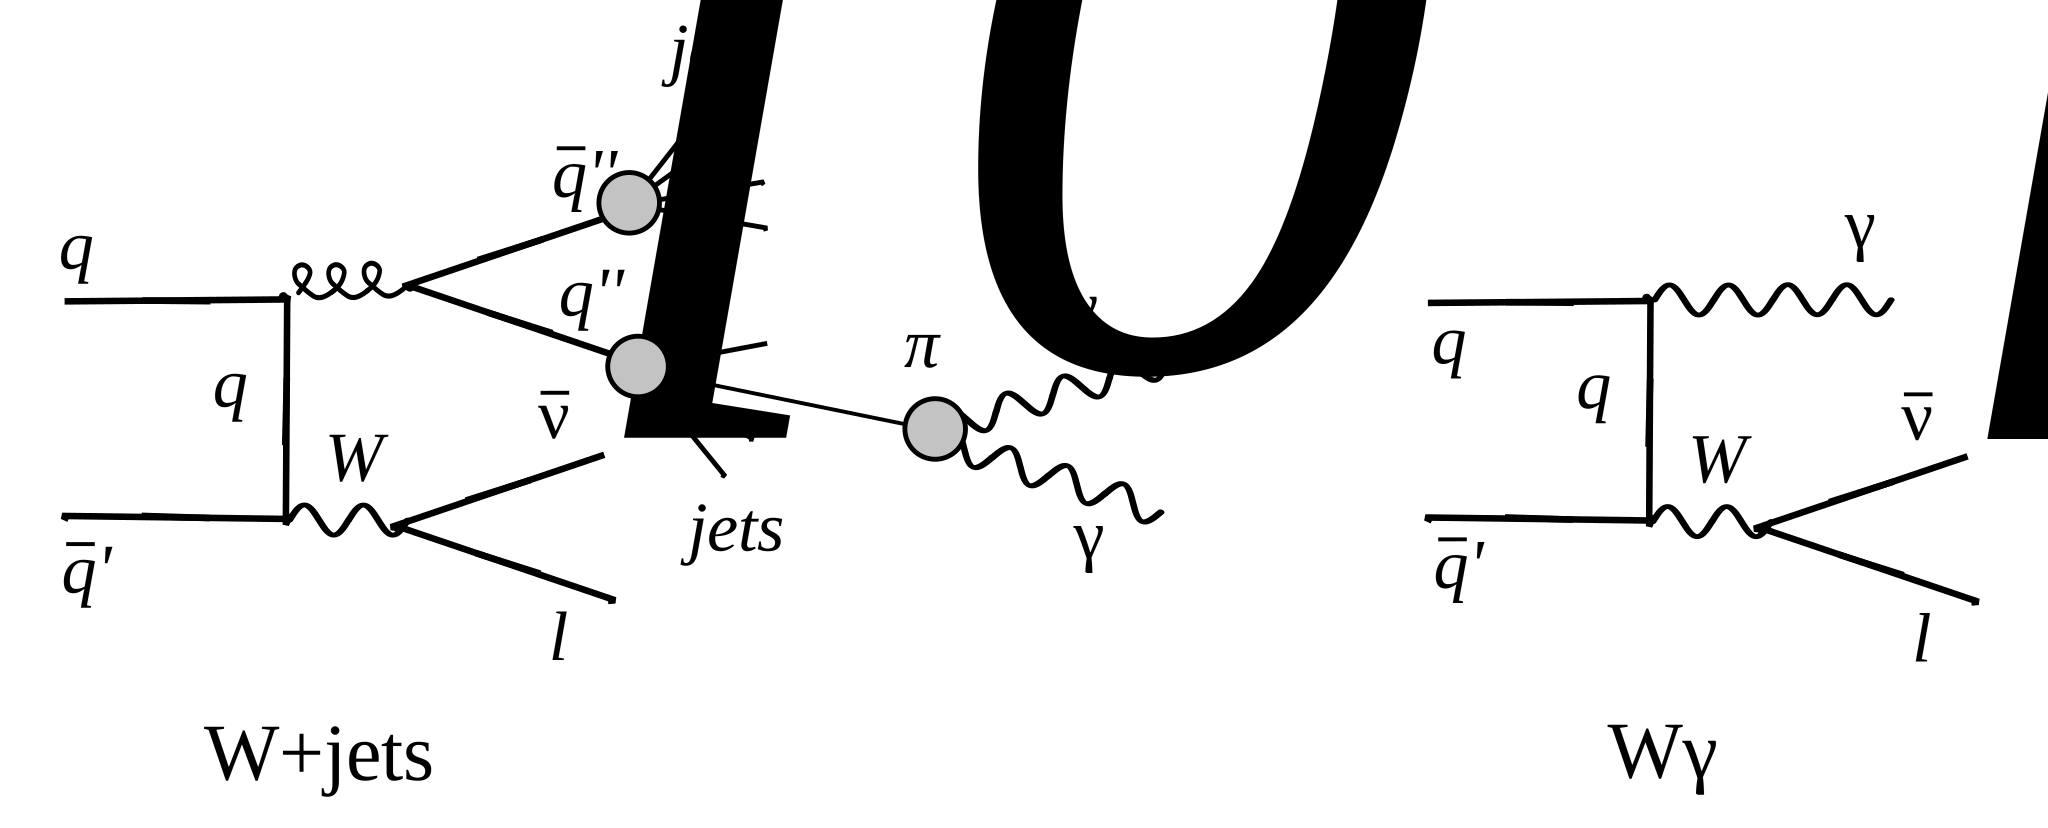
\includegraphics[width=0.95\textwidth]{../figs/ForPresentation/feynmWjets.png}}
  \end{center}
\end{figure}
  \scriptsize
  Jets$\rightarrow \gamma$: jets misidentified as photons.
  \tiny  
  Jets$\rightarrow \gamma$ background estimation is the most challenging part of this measurement and also the source of the largest systematic uncertainties (discussed later).
\end{frame}

\begin{frame}\frametitle{Jets$\rightarrow \gamma$ Background. Template Method}
 \tiny
  \begin{itemize}
    \item Choose a variable that has a significant discriminative power between the true-$\gamma$ and fake-$\gamma$ (jets$\rightarrow\gamma$) candidates $V_{fit}$;
    \item Prepare true-$\gamma$ ($T_{true}$) and fake-$\gamma$ ($T_{fake}$) templates {\tiny{(next slide)}};
    \item Fit $V_{fit}$ distribution in data by: $F(V_{fit})=N_{true} \cdot T_{true}(V_{fit}) + N_{fake} \cdot T_{fake}(V_{fit})$.
  \end{itemize}
\tiny
{\bfseries{Templates:}} accurate representations of $V_{fit}$ distributions of true-$\gamma$ and fake-$\gamma$ in the $W\gamma$-selected dataset.\\

\begin{minipage}[t]{0.49\textwidth}
  \begin{figure}[htb]
    \begin{center}
       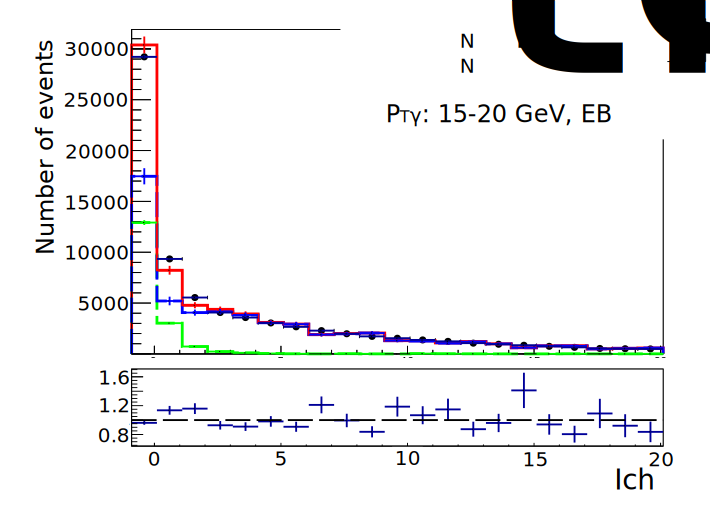
\includegraphics[width=0.98\textwidth]{../figs/ForPresentation/fitPlot_CHISO.png}
    \end{center}
  \end{figure}
    \begin{center}
       \tiny
       $V_{fit}=I_{ch}^{\gamma}$ (charged hadron isolation):\\
       $I_{ch}^{\gamma} = \sum P_T^{ch.had.}$, $\Delta R(\gamma,$ch.had.$)<$0.3\\
    \end{center}
\end{minipage}%
\begin{minipage}[t]{0.49\textwidth}
  \begin{figure}[htb]
    \begin{center}
      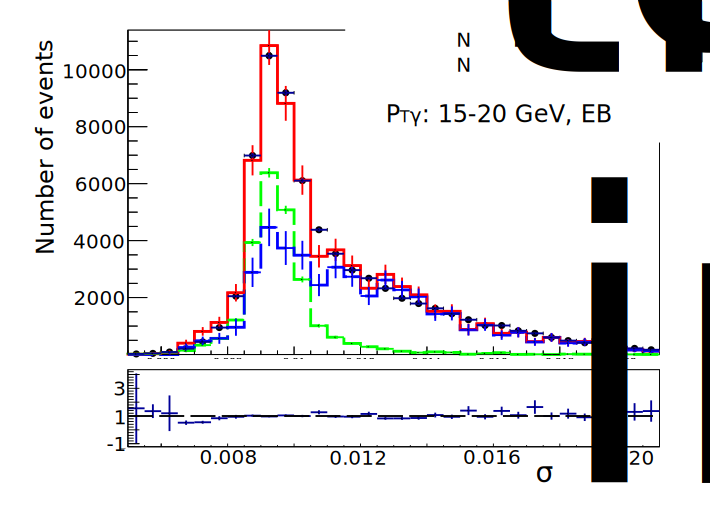
\includegraphics[width=0.98\textwidth]{../figs/ForPresentation/fitPlot_SIHIH.png}
    \end{center}
  \end{figure}
    \begin{center}
      \tiny
      $V_{fit}=\sigma_{i\eta i\eta}$: an ECal shower shape variable\\
    \end{center}
\end{minipage} 

\begin{center}
\tiny
Both $I_{ch}^{\gamma}$ and $\sigma_{i\eta i\eta}$ are used in photon ID.\\
\end{center}
{\bfseries{black}}: data; {\bfseries\color{green}{green}}: real-$\gamma$ template; {\bfseries\color{blue}{blue}}: fake-$\gamma$ template; {\bfseries\color{red}{red}}: fit function\\
{\bfseries{Note:}} fit results undergo a correction for $V_{fit}$ efficiency, and do not have to coincide before that. 
\end{frame}

\begin{frame}\frametitle{Jets$\rightarrow \gamma$. True-$\gamma$ Templates from $Z\gamma\rightarrow \mu^+ \mu^- \gamma $}

  \begin{figure}[htb]
      \begin{center}
        \scriptsize
          \includegraphics[width=0.95\textwidth]{../figs/ForPresentation/feynmZg_LO.png}
%          \caption{\scriptsize{The Feynman diagrams. ISR(x2), FSR, and TGC.}}
       \end{center}
    \end{figure}

\tiny
FSR: final state radiation; ISR: initial state radiation

  \begin{figure}[htb]
    \begin{center}
       \includegraphics[width=0.45\textwidth]{../figs/ForPresentation/forDefense_Mllg.png}\includegraphics[width=0.45\textwidth]{../figs/ForPresentation/forDefense_dR.png}\\
% \includegraphics[width=0.40\textwidth]{../figs/figs_v11/MUON_ZGamma/PrepareYields/c_TotalDATAvsMC_Endcap__MpholeplepVERY_PRELIMINARY_pt15to500_.png}\includegraphics[width=0.40\textwidth]{../figs/figs_v11/MUON_ZGamma/PrepareYields/c_TotalDATAvsMC_Endcap__lep1PhoDeltaRVERY_PRELIMINARY_pt15to500_.pdf}
    \end{center}
  \end{figure}
\tiny
$Z\gamma$-selected sample: $Z\gamma$ and $Z$+jets(DY+jets)\\
True-$\gamma$ templates: $M_{\mu\mu\gamma}<$101~GeV and $\Delta R(\mu_{1},\gamma)>$0.4 ($Z\gamma\rightarrow\mu^+ \mu^- \gamma $ FSR)\\

\end{frame}%{Jets$\rightarrow \gamma$. Real-$\gamma$ Templates from $Z\gamma\rightarrow{\bar{\mu}}\mu\gamma$}

\begin{frame}\frametitle{Jets$\rightarrow \gamma$. Fake-$\gamma$ Templates from $Z\gamma\rightarrow \mu^+ \mu^- \gamma$}

  \begin{figure}[htb]
    \begin{center}
       \includegraphics[width=0.45\textwidth]{../figs/ForPresentation/forDefense_Mllg.png}\includegraphics[width=0.45\textwidth]{../figs/ForPresentation/forDefense_dR.png}\\
% \includegraphics[width=0.40\textwidth]{../figs/figs_v11/MUON_ZGamma/PrepareYields/c_TotalDATAvsMC_Endcap__MpholeplepVERY_PRELIMINARY_pt15to500_.png}\includegraphics[width=0.40\textwidth]{../figs/figs_v11/MUON_ZGamma/PrepareYields/c_TotalDATAvsMC_Endcap__lep1PhoDeltaRVERY_PRELIMINARY_pt15to500_.pdf}
    \end{center}
  \end{figure}

\tiny
{\bfseries{$Z\gamma$-selected sample:}} $Z\gamma$, $Z$+jets; \\
{\bfseries{$W\gamma$-selected sample:}} $W\gamma$, $W$+jets, $Z$+jets, $t\bar{t}$+jets, and more\\

  \begin{itemize}
     \tiny
     \item Need $V_{fit}$ distributions of jets selected as photons (like in the $W\gamma$-selected sample);
     \item {\bfseries{Cannot find a pure sample of such jets in data;}}
     \item Use jets selected as photons in $Z\gamma \rightarrow \mu^+ \mu^- \gamma$-selected sample;
     \item Increase fake-$\gamma$ fraction: $M_{\mu\mu\gamma}>$101~GeV and $\Delta R(\mu_{1},\gamma)>$1.0 ($Z\gamma\rightarrow\mu^+ \mu^- \gamma$ ISR);
     \item {\bfseries{Sample is still dominant by true-$\gamma$ from $Z\gamma$ events}};
     \item Subtract the true-$\gamma$ contribution using $Z\gamma \rightarrow \mu^+ \mu^- \gamma$ simulation.
  \end{itemize}

\end{frame}%{{Jets$\rightarrow \gamma$ Background. Templates from $Z\gamma\rightarrow{\bar{\mu}}\mu\gamma$}
